\subsection{\href{http://www.digicard.com.ar/}{Digicard S.A.}}
   \hypertarget{subsec:digicard}
   For several years, I work for the company in the area of development of new hardware products aimed at access control. I can highlight the development of a new RFID reader of 125khz to replace the old magnetic cards readers and provide customized solutions integrated with the rest of the access control system of the company. I did the requirements, schematic design, PCB design, prototype, documentation for production, commissioning and documentation of use. The reader is still produced and using currently. Some photos of the equipment can be seen in figure \ref{fig:digicard}.
   \begin{figure}
      \begin{center}
         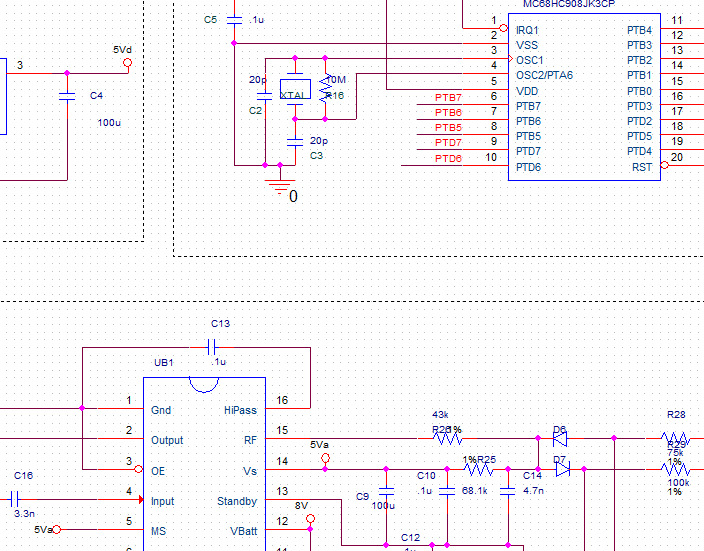
\includegraphics[width=0.24\textwidth]{digicard1.jpg}
         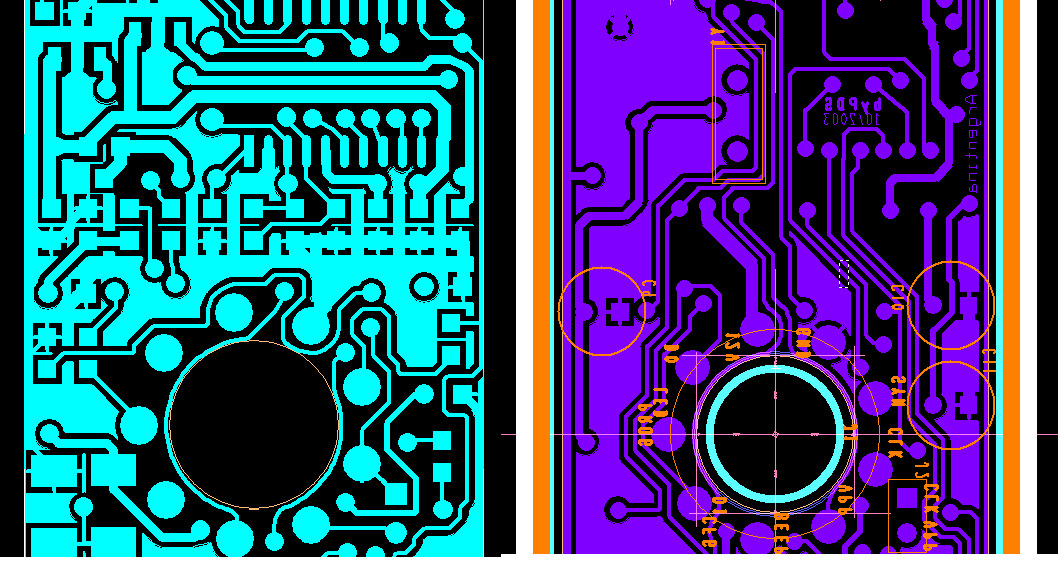
\includegraphics[width=0.24\textwidth]{digicard2.jpg}
         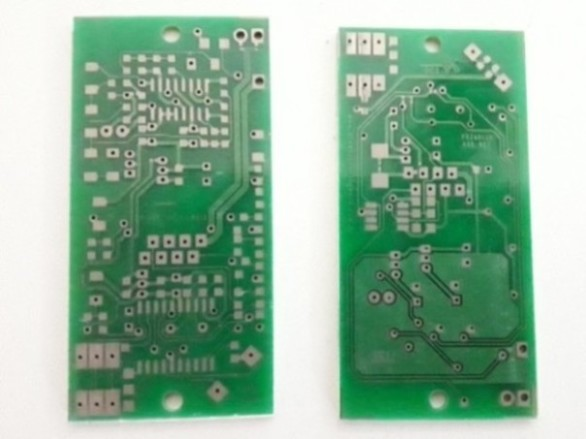
\includegraphics[width=0.24\textwidth]{digicard3.jpg}
         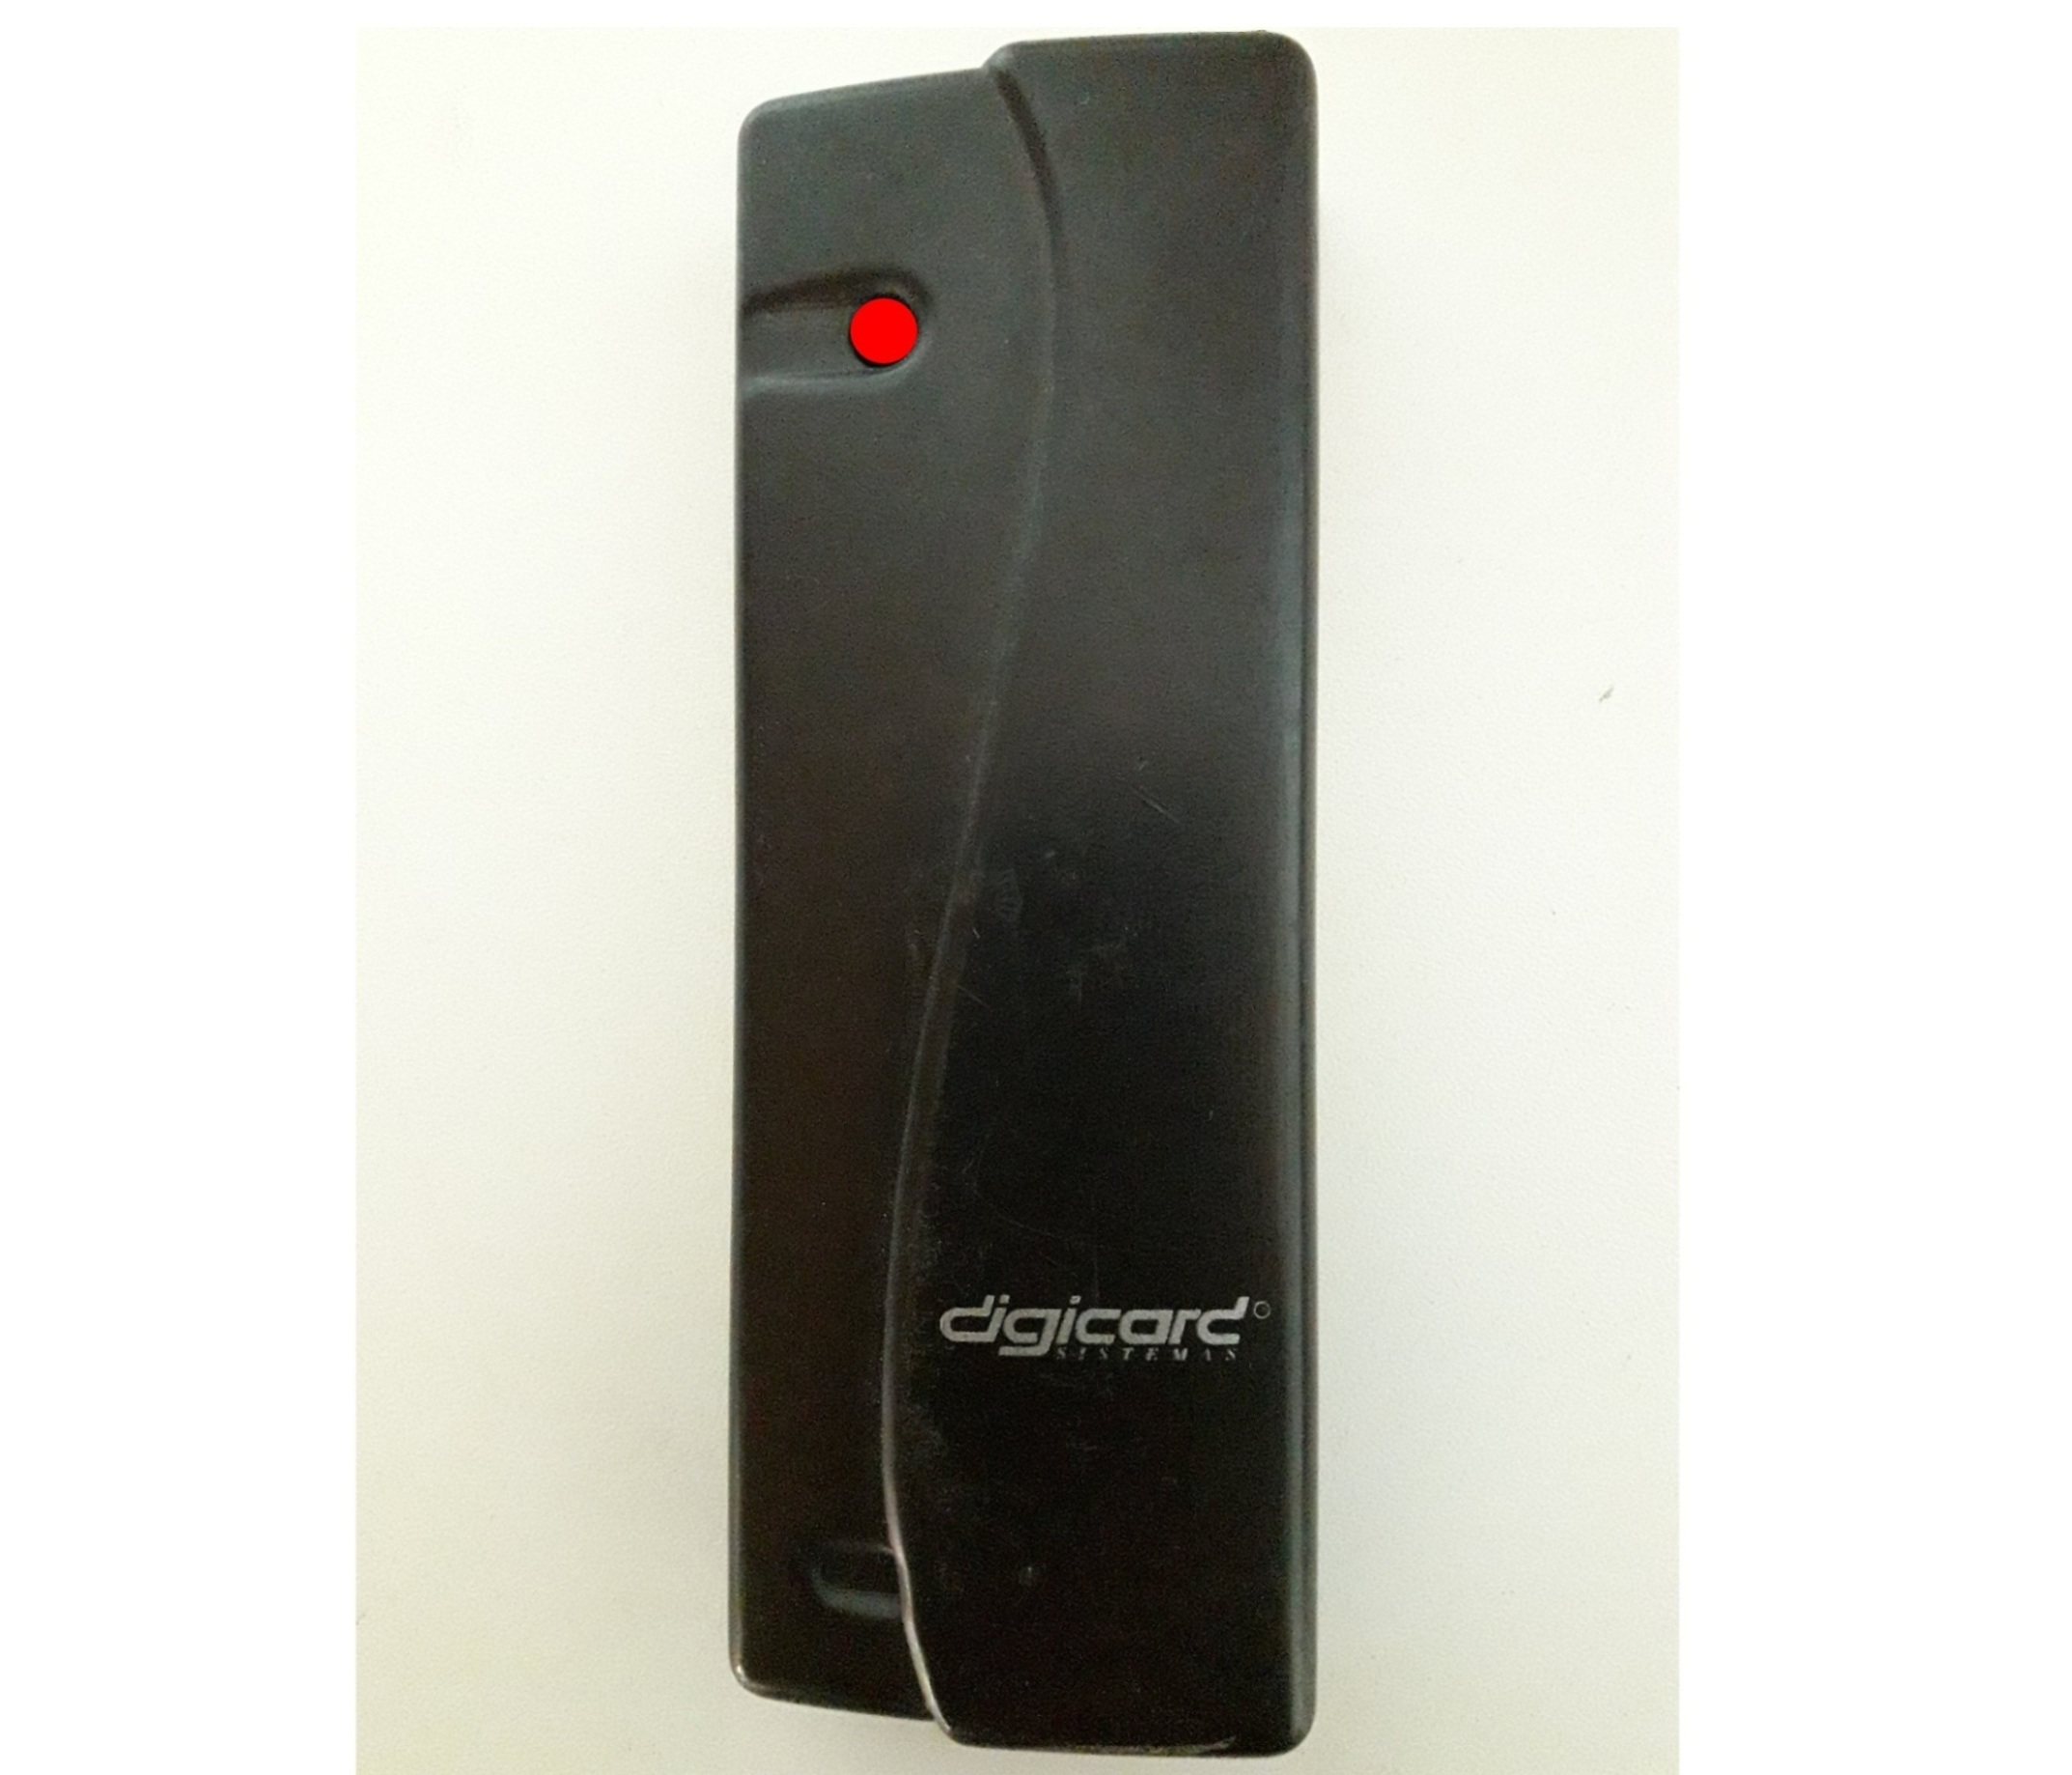
\includegraphics[width=0.24\textwidth]{digicard4.jpg}
      \end{center}
      \caption{Development of hardware, firmware and production of RFID reader of 125khz for the company Digicard.}
      \label{fig:digicard}
   \end{figure}
